After a model is trained, the first step is model selection and assessment.
Selection is estimating model performance among a set of \gls{ML} models using a
single validation set.  After one model is chosen, assessment takes place by
determining the prediction capability on new data via a previously unseen
testing set. Both selection and assessment can be done in a single step using
\textit{k}-fold cross-validation, which is described below.

\subsubsection{Sources of Error} 

In statistical learning, there are two sources of error that need to be
simultaneously minimized: bias and variance. Bias is caused by simplifications
in the model, so the error is caused by missed relationships in the data; high
bias is an indication of an underfit model.  Variance is caused by including
random noise in the model, so the error is caused by oversensitivity to that
noise; high variance is an indication of an overfit model. 

\begin{figure}[!htb]
  \makebox[\textwidth][c]{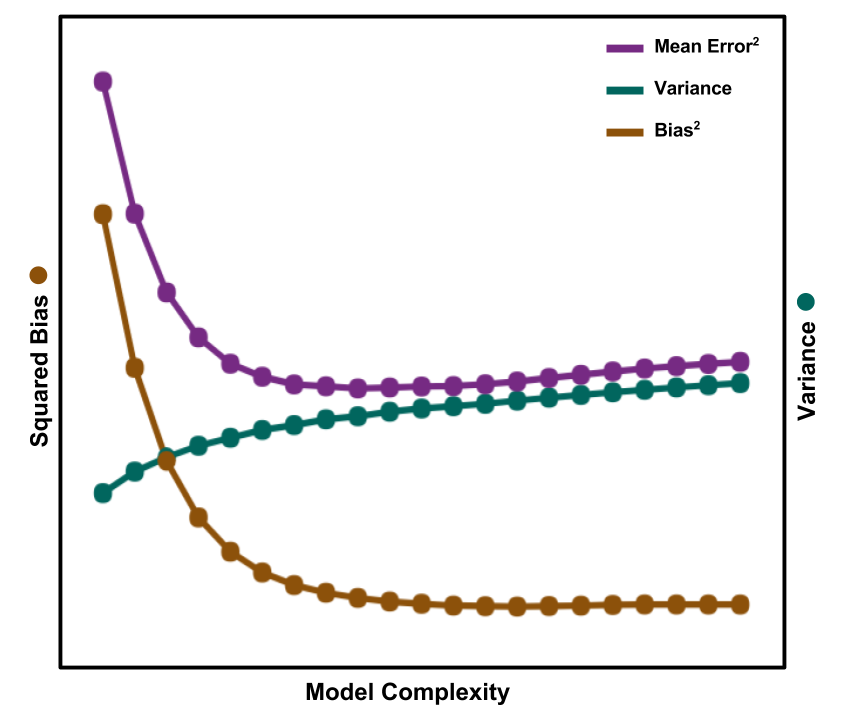
\includegraphics[width=\textwidth]{./chapters/litrev/BVtradeoff.png}}
  \caption{Bias and Variance Comprising Prediction Eror}
  \label{fig:bvtradeoff}
\end{figure}

Figure \ref{fig:bvtradeoff} shows the tradeoff between the bias and variance.
The shape of the total error curve has a minimum that we seek to achieve with
our model. Some bias is desired in order to generalize to future unknown data.
But some variance is also positive for the model because it captures the
relationships in the data that the bias counteracts. 

\subsubsection{Types of Error}

While the sources of the model prediction error are well known, the creation of
an \gls{ML} model is a hidden process. Although the model emerges
from a black box, there are ways to evaluate the generalization (i.e.,
prediction) capability of it.  This is done by removing a small portion of the
data for use as a testing set.  The rest of the data set is known as the
training set and is used to train a model. After training, the test set is used
to calculate the model's generalization error.  

Thus, the generalization error is typically referred to as the \textit{testing
error}, as it is measuring the ability of the model to predict future cases
that were not introduced in the training phase.
Next, the \textit{training error} is provided by comparing the model
predictions to the training set, as the model would likely be smoother than the
potential noise the training set would include. This is useful to determine the
fitness of the model, the application of which is discussed below in Section
\ref{sec:optvalid}.

Although one could just train and test their model, there is a way to check the
model while still in the training phase. A testing set that would be used
during training to give feedback, a \textit{cross-validation} set, can provide
a faster convergence to a satisfactory model. As shown in Figure
\ref{fig:cverror}, this can be done by splitting the data set into three
groups: a large training set, a small cross-validation set, and a small testing
set.  However, in practice, multiple rounds of cross-validation steps are used
provide the fastest convergence.  This is referred to as \textit{k-fold
cross-validation} and allows a user to have all training data entries be a
testing entry once, bettering model evaluation. 

\begin{figure}[!htb]
  \centering
  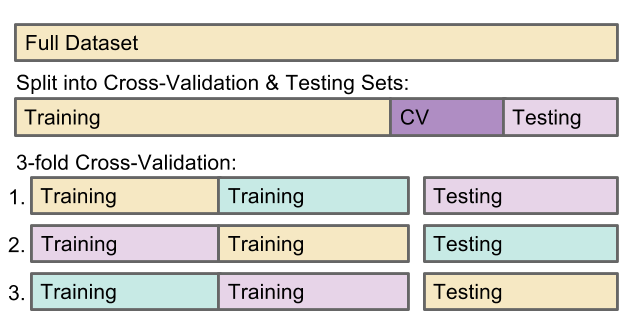
\includegraphics[width=0.85\linewidth]{./chapters/litrev/cverror.png}
  \caption{Illustration of Cross-Validation}
  \label{fig:cverror}
\end{figure}

Using cross-validation provides a \textit{cross-validation} error that replaces
the testing error during analysis.  As illustrated in Figure \ref{fig:cverror},
this splits the dataset into $k=3$ subsets. One set is designated as the
testing set, and a model is trained with the rest. Following the first training
phase, another begins, this time with a different subset as the testing set.
In total, this process in Figure \ref{fig:cverror} is performed $3$ times,
giving $3$ models. The metrics of model performance are averaged by taking the
mean of the accuracy/error of predictions.  This provides an additional level
of model validation than can be achieved with a single testing set. This mean
is reported as the cross-validation error. If the cross-validation error is
acceptable, then training is performed on the entire training data set and can
be tested on new observations.
